\subsection{MAPC: Contest and Scenario}
\todo{Write this section}
What is the general scenario? Agents on mars trying to find water in a competitive manner against another team. Explain the concept of zones, gaining points, achievements and also how agents differ from each other. Introduce the notion of \emph{zoning} as the process of finding and forming a zone (including upkeeping by defense?).
I've put this section first so the later chapters can already rely on the reader knowing what the scenario is about. Furthermore, we can then directly rule out concepts which we are presenting by applying them theoretically onto the scenario/our needs.

\subsection{Agent Programming Concepts}
\todo{Write this section}
\subsubsection[BDI]{BDI$^\blacktriangle$}
Using cognitive modelling techniques for simulating human behaviour, without requiring people interactions can save a lot of people forces, resources, time and money. So that a variety of researchers are contributing to intelligent agents field. Beliefs, desires and intentions (BDI) agent is a kind of intelligent agent. BDI model describes the basic characteristics of agents' mental state since the BDI logic system is easy to be realised in the computer, and has been wildly applied in these fields. In recent years, many scholars have used Java, Jason or some other languages to implement BDI agent model in computer.

In 1987, Bratman\cite{MICHAEL_PlansResource_1988} discussed the relationship among beliefs, desires, intentions and actions as well as considering that they play important roles in option behaviours. This is the foundation of BDI model and BDI logic. In 1991, Rao and Georgeff\cite{Michael_BDIAgency_1999} modelled the BDI agent behaviour and treated beliefs, desires and intentions as three modal operators and applied BDI agent to airline traffic management. Nowadays, the research on BDI agents are not only used in high value domains but also in daily lives. We can see the applications are not only in high technology industrial aspect as air-plane or space shuttle but also in commercial field or entertainment such as robot soccer games.

The BDI model is a popular and well-studied architecture of agent for intelligent agents situated in complex and dynamic environments. The model has its roots in philosophy with Bratman’s theory of practical reasoning\cite{Sebastian_Hierarchical_2006}. Practical reasoning involves two important processes: deciding what goals we want to achieve, and how we are going to achieve these goals. The former process is known as deliberation, the latter as means-ends reasoning\cite{Gerhard_MultiSystem_1999}. When an agent is placed in an environment, it should decide what to do and how to do. There are a lot of options of affairs states, but not all of them are good choices. Some other affairs more or less have influences on the feasibility of achieving these goals. The deliberation process is to understand and filter what options are available, in addition, generate the set of alternatives which will be chosen as following. These chosen options become intentions which can be treated as the outputs of deliberation. For example, if you are standing in a supermarket and very thirsty, then you are faced with a decision to choose a drink. There are a lot of options like wine, beers, milk, water and juice, however, picking up a bottle of wine is not available to you if you are younger than 18 years old. After collecting all the available options, you must choose and commit to some of them which become intentions next. Subsequently, we need the mean-ends reasoning process to plan how to achieve these intentions. Furthermore, your intention is to buy a bottle of water, then you plan to go to the shelf with water on it, and stretch your arm to get a bottle of water on the top. Finally, you execute this plan to get a water.

As a theory of practical reasoning, BDI model has three attributes that are belief, desire and intention.

% TODO BDI three attributes
Beliefs represent the informational state of the agent and be updated appropriately after each sensing action.They may be implemented as a variable, a database, a set of logical expressions, or some other data structure\cite{Rao_BDITheory_1995}. Belief means how the agent look at the world and it is the basis of BDI model. Belief includes the information about environment, other agents and itself. An agent needs to be allowed to update its beliefs at any time. Updating information comes from the perception of the environment, and the execution of intentions. An agent can use sensors to perceive the environment to get signals to believe. In addition, after executing some intentions, these become the information believed by the agent. Belief is not the same concept as knowledge. Beliefs are only required to provide information on the likely state of the environment, but knowledge is the realisation of a fact. Beliefs are just the state believed by agents but no one can ensure what they believe are true. Simple to say, knowledge is true belief.

Desires represent the motivational state of the agent\cite{Rao_BDITheory_1995}. They represent objectives or situations that the agent would like to accomplish or bring about. They are state of affairs that the agent would wish to bring about or to keep. Desires may be achieved or never achieved, and it doesn't need to believe that desires must be achieved. Desires are different from goals although they look pretty similar. Desires can be inconsistent and the agent need not know the means of achieving these desires. Desires have the tendency to 'tug' the agent in different directions. They are inputs to the agent's deliberation process, which results in the agent choosing a subset of desires that are both consistent and achievable. Such consistent achievable desires are usually called goals\cite{Gerhard_MultiSystem_1999}. For example, sleeping and working may be both my desires, but they can not be my goals at the same time because they have conflicts.

Intentions are desires or actions that the agent has committed to achieve\cite{Alejandro_LearnBDI_2004}. Intentions are stronger than desires. Desires are just wishes that may be achieved or may be not, but intentions to an extent are decided to be achieved. Michael Wooldridge concluded four roles of intentions playing in practical reasoning. The roles are intentions drive means-ends reasoning; intentions constrain future deliberation; intentions persist and intentions influence beliefs upon which future practical reasoning is based\cite{Gerhard_MultiSystem_1999}. Intentions driving means-ends reasoning means that intentions have decisive influences on actions the agent will execute. Agents are expected to determine ways of achieving intentions. Intentions constraining future deliberation means that options that are inconsistent with this intention will not be entertained. intentions persisting means that intentions will be never given up unless the reason is rational.As we know, intentions are committed desires which can not be easily abandoned. For if I immediately drop my intentions without devoting resources to achieving them, then I will never achieve anything\cite{Gerhard_MultiSystem_1999}. But when a good reason exists, I still can drop intentions instead of persisting them for a long time without achievement. If it is very clear that the intentions will never been achieved, then there is no need to keep them. Similarly, if the reason for intention is no longer true, then intentions should be given up. Another reason of dropping intentions is the intentions have been achieved already. Intentions influencing beliefs upon which future practical reasoning is based means that believing intentions will be achieved. If I adopt an intention, then I can plan for the future on the assumption that I will achieve the intention. For if I intend to achieve some state of affairs while simultaneously believing that I will not achieve it, then I am being irrational\cite{Gerhard_MultiSystem_1999}. Agents should believe that they believe there is at least some way that the intentions could be brought about and believe that under "normal circumstances" agents will succeed with the intentions, or say it in another way, agents do not believe they will not bring about their intentions. Generally speaking, intentions are not random ideas, but the wants to a reasonable extent. It plays an important role in BDI model that leading to actions, constraining future deliberation and influencing future beliefs. Specifically, the agents should drop off some intentions at times to avoid resource wasting. It is necessary to keep a good balance between these different concerns.
\todo{For some reason, the spacing here between paragraphs seems to increase at times. I haven't quite figured out why and when this happens.}

Beliefs, desires and intentions are three attributes of BDI model and constitute the foundation of BDI agents. While, some other components building connection between beliefs, desires and intentions are also indispensable to implement BDI agents and make the BDI architecture completed.
% TODO BDI basic architecture//pic
Several basic components can be found in the following figure, which is a brief BDI architecture. A variety of BDI agents have been designed to fit the unstable environment and to complete all sorts of tasks. Different BDI agents have different architectures, but their core ideas are same.

\begin{figure}[htbp]
  \centering
  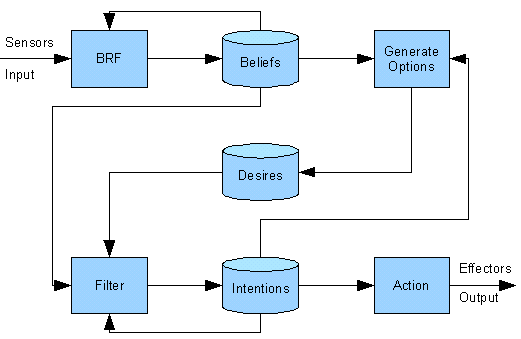
\includegraphics[width=\textwidth]{images/BDIAr}
  \caption{Brief BDI architecture \cite{BDIA}}%use cite instead
  \label{fig:Brief BDI architecture}
\end{figure}

The sensors of the BDI agent perceive the environment and convert the perceptions to signals as the inputs to the belief revision function. It will collect the perceptions from outside as well as the beliefs which are stored in the beliefs set. After mapping the information, computing and revising using belief revision function, the new beliefs will set into the beliefs set. The belief revision function prefers minimal change rather than modifying a lot. There are not big differences between the revised beliefs set and the previous one to preserve as much information as possible by the change\cite{M_Belief}. The belief revision function is used to keep the beliefs set being updated to fit the unstable environment, on the other hand, it can avoid the inconsistent situations occurring among those beliefs like the agent believes what it doesn't believe.

The beliefs set contains information about the current environment which the agent has. The data in beliefs set may be sentences, rules or some other manifestations. In the AGM (named after the names of their proponents, Alchourrón, Gärdenfors, and Makinson)\todo{@yuansun1990: I couldn't find it quickly but please link to the original work introducing AGM as well. And naturally, also quickly look over it so you know that your statements are correct.} approach, an agent’s beliefs are modelled by a deductively closed set of formulas called a belief set\cite{James_revise_2011}.
The current set of beliefs is represented by a deductively closed set of logical formulae K called belief base, the new piece of information is a logical formula P, and revision is performed by a binary operator * that takes as its operands the current beliefs and the new information and produces as a result a belief base representing the result of the revision\cite{M_Belief}. Many researchers are doing researches in belief revision using AGM approach.
The option generator reads the beliefs information and returns a list of options which are current desires into the desires set. It determines the desires depending on the agent’s current beliefs and current intentions. The desires set contains many desires are possible courses of actions available to the agent, and These desires can be no matter achieved or not. The filter determines the agent’s intentions depending on current beliefs, desires, and intentions. It needs to consider about more situations than the functions in previous steps. Desires will become more rational after filtering.

The intentions set stores the agent’s current focus, which are going to be executed or committed to be executed at some time. Once an intention is adopted, it should not be immediately dropped out because of the commitment. But in some situations, the intentions should be given up depending on  three commitment strategies having been proposed in Rao and Georgeff’s work:  blind, single minded and open minded. A blindly committed agent is an agent who maintains his intentions until he believes that he has achieved them. A single minded committed agent is an agent who maintains his intentions as long as he believes that they are still options. An open minded committed agent is an agent who maintains his intentions as long as they are still goals\cite{Roberto_BDIATL_2005}. The action selection function determines the actions to perform depending on current intentions. We would achieve nothing if we just have intentions instead of knowing how to do it. Normally, there is a plan library of mapping between the intentions and actions. The intentions go through the planner and the actions which mapping the corresponding intentions are founded. At last, a plan of how to achieve the intentions come out and the agent will execute these actions.

For understanding the relationships between the seven main components of BDI agent architecture, one table is presented as followed:

\begin{table}[!hbp]
  \label{tab:BDIC}
  \begin{tabularx}{\textwidth}{|l|p{5cm}| >{$}X<{$} |}
  \hline
  \textbf{Component} & \textbf{Meaning} & \textbf{Formalisation} \\
    \hline
    Beliefs set & Information about the current environment which the agent has & B \\
    \hline
    Belief revision function & determines a new set of beliefs depending on perceptual inputs and the agent’s current beliefs & B \times P \to B\\
    \hline
    Options & determines desires depending on the agent’s current beliefs & B \times I \to D \\
    \hline
    Desires set & possible courses of actions available to the agent & D \\
    \hline
    Filter & determines the agent’s intentions depending on current beliefs, desires, and intentions & B \times I \times D \to I \\
    \hline
    Intentions set & the agent’s current focus & I \\
    \hline
    Action selection function & determines an action to perform depending on current intentions & I \to A  \\
    \hline
  \end{tabularx}
  \caption{Components of brief BDI agent architecture}
\end{table}

This table shows the order of using the seven components of BDI architecture as well as giving the formulas of each function. There, $Bel$ is a set of all possible beliefs, $Des$ is a set of all possible desires and $Int$ is a set of all possible intentions. Therefore, an agent state can be presented as $(B,D,I)$ with $B \subseteq Bel, D \subseteq  Des, I \subseteq  Int$. $P$ is a set of current perception which are obtained by the sensors of the agent. we can understand the the process of BDI agent working better through seeing this table. Firstly, $B$ has stored some beliefs which are read by BRF while it getting the perception from the sensors. After operating BRF, some of beliefs are removed, some are added, some are modified and so on. So the new beliefs set $B$ built on basis of $P$ and original $B$. Subsequently, Options use the new $B$ and current Intentions set $I$ to determine the desires set $D$ and store it. Moreover, the filter select intentions by referencing $B,D,I$, then the new intentions set comes out. Finally, the action selection function makes a plan to execute actions to achieve $I$.

The process of $B \times P \to B$, $B \times I \to D$ and $B \times I \times D \to I$ belongs to deliberation. They are deliberated in-depth gradually and the range of intentions are narrowed, especially the filter which should consider of all there datasets. At last, the intentions are limited in particular ranges. The plans will be made more effective and more targeted.  $I \to A $ can be treated as the process of means-ends reasoning, whose output is planning. $B,D I$ are connected to function parts instead of connecting to each other directly. They are just databases and need rules or mechanism to help them execute actions.

% TODO BDI applications (short)
With the increasing needs of intelligent agents, more and more applications base on BDI model are applied in our life. PRS and dMARS are both BDI-based systems for the reaction control system of the NASA Space Shuttle Discovery. Additionally, an air-traffic management system, OASIS, is well-known as a BDI-dased agent. The system architecture for OASIS is made up of one aircraft agent for each arriving aircraft and a number of global agents including a sequencer wind modeller coordinator and trajectory checker\cite{Rao_BDITheory_1995}. Furthermore, robot soccer which are designed using BDI model becomes very popular in universities. We can feel that, BDI agents bring many profits to human beings, they make the life more convenient. However, it still has development space in this field.

Although the BDI model is developed during about 30 years, some obstacles are not overcome and some challenges are still there. Most BDI implementations do not have an explicit representation of goals. The agents should reason the goals from the current beliefs and intentions. Besides, the BDI model contains three attributes, beliefs, desires and intentions. In some situations, not all the three attributes are needed. Sometimes, an agent collect the beliefs and jump to intentions directly without desires. However, for some distributed multi-agents, just three attributes are not sufficient to execute the actions.  Furthermore, the agents in the multi-agents system don't have a explicit mechanisms for interaction and integration among them. When an increasing number of agents join the system, the interaction with each agent will be more and more difficult. As an intelligent agent, the BDI agent don't have a good ability to learning from from past behavior or other agents’ behavior. So that the rate of development will not be high if lack mechanisms to learn from others. However, BDI model has its own advantages. Beliefs, desires and intentions are similar to the mental activities of human beings. Therefore, it is not easy to construct the logics or mechanisms for it. With the wildly used of computers and mobile devices, the situation of multi-agent interaction will be better. As many computer languages and logic languages are grasped by more people, the BDI agent will bring human beings more surprises.

An introduction of beliefs, desires and intentions model is presented in this section. The BDI agent belongs to intelligent agent which are autonomous, computational entities. The BDI agent executes actions on the basis of BDI model that containing three main attributes which have close relationship with each other. The brief BDI agent architecture is a clear description of process of BDI agents work. And They follows the practical reasoning theory. Different BDI implements show different architectures, but the core idea of these agents are still beliefs, desires and intentions. With an increasing number of BDI applications go into the humans life, more challenges come up too. The BDI model has its own advantages and disadvantages, but I still believe that it can bring more surprises to own life in the future.





\subsubsection[Formal Methods]{Formal Methods$^\diamond$}
As was mentioned in ~\autoref{fun:BDI}, usage of BDI agents brings up several challenges.
One of the important challenges of multi-agent systems is to make sure that the agent will not behave in an unacceptable or undesirable way.
Agents may act in complex production environments, where failure of a single agent may cause serious losses.
Formal methods have been used in computer science as a basis to solve correctness challenges.
They represent agents as a high-level abstractions in complex systems.
Such a representation can lead to simpler techniques for design and development.

There are two roles of formal methods in distributed artificial intelligence that are often referred to.
Firstly, with respect to precise specifications they help in debugging specifications and in validation of system implementations.
Abstracting from specific implementation leads to better understanding of the design of the system being developed.
Secondly, in the long run formal methods help in developing a clearer understanding of problems and their solutions. \cite{Singh_99}

To formalise the concepts of multi-agent systems different types of logics are used, such as propositional, modal, temporal and dynamic logics.
In the following several paragraphs these logics, their properties and introduced operators will be briefly discussed.
Describing the details of interpretations and models of each individual logic is not the purpose of this report and is left out for further reading.

Propositional logic is the simplest logic and serves as the basis for logics discussed further in this section.
It is used to represent factual information and in our case is most suitable to model the agents' environment.
Formulas in this logic language consist of atomic propositions (represinting known facts about the world) and truth-functional connectives: $\land,\lor,\neg,\rightarrow$ which denote \enquote{and}, \enquote{or}, \enquote{not} and \enquote{implies}, respectively~\cite{Enderton_72}.

Modal logic extends propositional logic by introducing two different modes of truth: possibility and necessity.
In the study of agents, it is used to give meaning to concepts such as belief and knowledge.
Syntactically, modal operators in modal logic languages are defined as $\Diamond$  for possibility and $\Box$ for necessity.
The semantics of modal logics are traditionally given in terms of sets of so-called \emph{possible worlds}.
A world here can be interpreted as a possible state of affairs or sequence of states of affairs (history).
Different worlds can be related via a binary accessibility relations, which tells us which worlds are within the realm of possibility from the point of view of a given world.
In the sense of the accessibility relation, a condition is assumed \emph{possible} if it is true somewhere in the realm of possibility and it is assumed \emph{necessary} if it is true everywhere in the realm of possibility~ \cite{Saul_63}.

Dynamic logic is also referred to as modal logic of action.
It adds different atomic actions to the logic language.
In our case, atomic actions may be represented as actions that agents can perform directly.
This makes dynamic logic very flexible and useful for distributed artificial intelligence systems.
Necessity and possibility operators of dynamic logic are based upon the kinds of actions available~\cite{Kozen_90}.

Temporal logic is the logic of time.
There are several variations of this logic, such as:
\begin{description}
  \item[Linear] (or \emph{branching}): single course of history or multiple courses of history.
  \item[Discrete] (or \emph{dense}): discrete steps (like natural numbers) or always having intermediate steps (like real numbers).
  \item[Moment-based] (or \emph{period-based}): atoms of time are points or intervals.
\end{description}
We will concentrate on discrete moment-based models with linear past, but consider both linear and branching futures.

Linear temporal logic introduces several important operators. $p\cup q$ is true at a moment $t$ on a path, if and only if $q$ holds at a future moment on the given path and $p$ holds on all moments between $t$ and the selected occurrence of $q$.
$Fp$ means that $p$ holds sometimes in the future on the given path.
$Gp$ means that $p$ always holds in the future on the given path.
$Xp$ means that $p$ holds in the next moment.
$Pq$ means that $q$ held in a past moment~\cite{Singh_99}.

\begin{figure}[h!]
  \caption{An example branching structure of time~\cite{Singh_99}.}
  \centering
  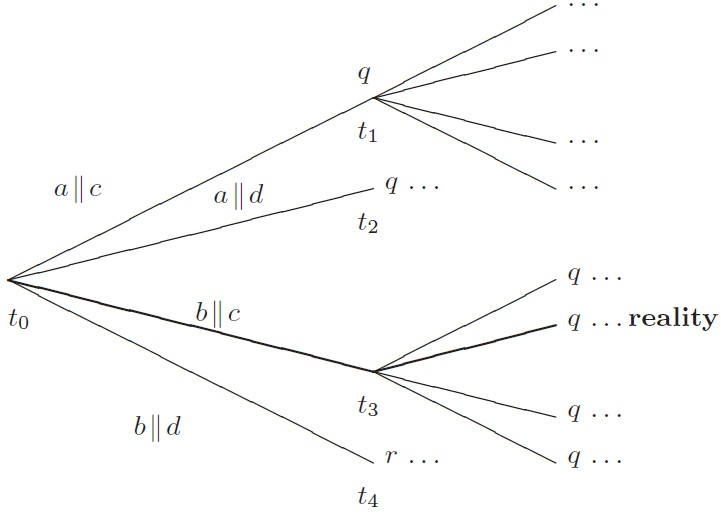
\includegraphics[width=0.6\textwidth]{images/branching_logic.png}
  \label{fig:for_branching_figure}
\end{figure}

Branching temporal and action logic is built on top of both dynamic and linear temporal logics and captures the essential properties of actions and time that are of value in specifying agents.
It also adds several specific branching-time operators.
$A$ denotes \enquote{in all paths at the present moment}.
The present moment here is the moment at which a given formula is evaluated.
$E$ denotes \enquote{in some path at the present moment}.
The reality operator $R$ denotes \enquote{in the real path at the present moment}.
\autoref{fig:for_branching_figure} illustrates the example of branching time for two interacting agents.

For modeling intelligent agents, quite often the BDI concept is used, which was described earlier in this report.
BDI stands for three cognitive specifications of agents: beliefs, desires and intentions.
To model logic of these specifications we will need to introduce several modal operators: $Bel$ for beliefs, $Des$ for desires, $Int$ for intentions and $K_h$ for know-how.
Considering these operators, for example, the mental state of an agent who desires to win the lottery and intends to buy a lottery ticket sometime, but does not believe that he will ever win can be represented by the following formula: $DesAFwin \land IntEFbuy \land \neg BelAFwin$.
For simplification in future we will consider only those desires which are mutually consistent.
Such desires are usually called goals.

It is important to note several important properties of intentions, which should be maintained by all agents~\cite{Singh_92}:
\begin{description}
  \item[Satisfiability] $xIntp\rightarrow EFp$.
    This means that if $p$ is intended by $x$, then it occurs eventually on some path.
    An intention following this condition is assumed to be satisfiable.
  \item[Temporal consistency] $(xIntp \land xIntq)\rightarrow xInt(Fp \land Fq)$.
    This requires that if an agent intends $p$ and intends $q$, then it (implicitly) intends achieving them in some undetermined temporal order: $p$ before $q$, $q$ before $p$, or both simultaneously.
  \item[Persistence does not entail success] $EG((xIntp) \land \neg p)$ is satisfiable.
    This is quite intuitive: just because an agent persists with an intention does not mean that it will succeed.
  \item[Persist while succeeding] This constraint requires that agents desist from revising their intentions as long as they are able to proceed properly.
\end{description}

The concepts introduced above may be used in each of the two roles of formal methods introduced earlier.
The two most commonly used reasoning techniques to decide an agent's actions are theorem proving and model checking.
The first one is more complex in terms of calculations, when the second one is more practical, but it requires additional inputs, though it does not prove to be a problem in several cases.

Considering the practical implementation, the architecture of an abstract BDI-interpreter can be described as follows.
The inputs to the system are called events, and are received via an event queue.
Events can be external or internal in relation to the system.
Based on its current state and input events, the system selects and executes options, corresponding to some plans.
The interpreter continually performs the following: determine available options, deliberate to commit to some options, update the state and execute chosen atomic actions.
After that, it updates the event queue and eliminates the options which have already achieved or are no longer possible.

\todo{Add or leave out a caption for all listings. Currently we are not consistent with that.}
\begin{lstlisting}[caption={An abstract BDI interpreter~\cite{Singh_92}.}]
  BDI-Interpreter
  initialise_state();
  do
    options := option-generator(event-queue, B, G, I);
    selected-options := deliberate(options, B, G, I);
    update-intentions(selected-options, I);
    execute(I);
    get-new-external-events();
    drop-successful-attitudes(B, G, I);
    drop-impossible-attitudes(B, G, I);
  until quit.
\end{lstlisting}

As was mentioned above, options are usually represented by plans.
Plans consist of the name or type, the body usually specified by a plan graph, invocation condition (triggering event), precondition specifying when it may be selected and add list with delete list, specifying which atomic propositions to be believed after successful plan execution.
Intentions in this case may be represented as hierarchically related plans.

Getting back to the algorithm and assuming plans as options, the option generator may look like the following.
Given a set of trigger events from the event queue, the option generator iterates through the plan library and returns those plans whose invocation condition matches the trigger event and whose preconditions are believed by the agent.

\begin{lstlisting}[mathescape, caption={Option generation for BDI interpreter~\cite{Singh_92}.}]
  option-generator(trigger-events, B, G ,I)
  options := {};
  for trigger-event $\in$ trigger-events do
    for plan $\in$ plan-library do
      if matches(invocation(plan, trigger-event) then
        if provable(precondition(plan), B) then
          options := options $\cup$ plan;
  return options.
\end{lstlisting}

Deliberation of options should conform with the execution time constraints, therefore under certain circumstances random choice might be appropriate.
Sometimes lengthy deliberation becomes possible by introducing meta-level plans into the plan library, which form intentions towards some particular plans.

\begin{lstlisting}[mathescape, caption={Option deliberation for BDI interpreter~\cite{Singh_92}.}]
  deliberate(options)
  if length(options) $\leq$ 1 then return options;
  else metalevel-options :=
            option-generator(b-add(option-set(options)));
    selected-options := deliberate(metalevel-options);
    if null(selected-options) then
        return random-choice(options);
    else return selected-options.
\end{lstlisting}

Coordination is one of the core functionalities needed by multi-agent systems.
Especially when different agents act autonomously and have different roles and possible actions.

One of the approaches developed by Singh~\cite{Singh_97} represents each agent as a small skeleton, which includes only the events or transitions made by the agent that are significant for coordination.
The core of the architecture is the idea that agents should have limited knowledge about the designs of other agents.
This limited knowledge is called the significant events of the agent.
There are four main types of events:
\begin{itemize}
  \item flexible, which can be delayed or omitted,
  \item inevitable, which can only be delayed,
  \item immediate, which the agent is willing to perform immediately,
  \item triggerable, which the agent performs based on external events.
\end{itemize}
These events are organised into skeletons that characterise the coordination behavior of agents.
The coordination service is independent of the exact skeletons or events used by agents in a multi-agent system.

To specify coordinations, a variant of the linear-time temporal language with some restrictions is used.
Two temporal operators are introduced for this purpose: $\cdot$, which is the before operator, and $\bigodot$, which is the operator of concatenation of two time traces, the first of which is finite.
Such special logic allows a variety of different relationships to be captured.

Overall, formal methods provide a logic abstraction for multi-agent systems.
They help to find self-consistent models of an agent's behavior.
However, relatively high complexity does not allow these methods to be implemented in real-time systems.
Therefore, the role of formal methods nowadays is limited to debugging, validation and design purposes.

In our project we unfortunately did not apply any formal methods for debugging or validating, mostly because of the limited time for development.


\subsubsection[Negotiation and Argumentation]{Negotiation and Argumentation$^\diamond$}
In multi-agent environment, where each agent has its own beliefs, desires and goals, achieving a common goal usually require some sort of cooperation. It most of the cases it can be achieved through communication and negotiation among groups of agents. Often negotiation is supported by some arguments which help to identify which agent is more suitable for completing certain task. Among them could be better position, better resources for completing the task, importance of current goal and so on. Some arguments can be also used to change the intentions of other agents. This could be the arguments like reserving the node to explore or the enemy to attack and many others. Argumentation is essential when agents don't have the full knowledge about other agents or environment. In such cases exchanging information helps to develop the consensus and make cooperative decisions.

To negotiate effectively a BDI agent requires the ability to represent and maintain the model of its own properties, such as beliefs, desires, intentions and goals, reason with other agents' properties and be able to influence other agent's properties \cite{Kraus_98}. These requirements should be supported by the agent programming language we choose for our project. 

As was mentioned above, negotiation is performed through communication. Negotiation messages can be of the following three types: a request, response, or a declaration. A response can take the form of an acceptance or a rejection. Messages can also have several parameters for justification or transmitting negotiation arguments. The arguments are produced independently by each agent using the predefined rules, which will be discussed later in this subchapter. Every agent can send and receive messages. Evaluating a received message is the vital part of negotiation procedure. Only the evaluation process following an argument may change the core agents' beliefs, desires, intentions or goals. 

There are always several ways of modelling agents for negotiation. Agents can be bounded if they do not believe in "false"; omniscient if their beliefs are closed under inferences; knowledgable if  their beliefs are correct; unforgetful if they never forget anything; memoryless if they do not have memory and they cannot reason about past events; non-observer if their beliefs may change only as a result of message evaluation; cooperative if they share the common goal \cite{Kraus_98}. For our project in most of the cases we assumed agent as knowledgable and memoryless - agents remember only about the current round of negotiation and abolish previous round results, when the new round starts. During the zone building process the agents also act as cooperative, since they share the common goal of building a zone.



\subsubsection{Agent Societies}
\todo{add, adapt and improve Rahul's part if it fits and is helpful for our later work}
\subsection[Agent Programming Languages]{Agent Programming Languages$^\circ$}
We investigated several agent programming languages, for their suitability for the \mars scenario.
Our goal was to determine which specialised language we wanted to use for multi-agent programming, if any.
The following sections present the basic structure of various languages together with examples.
These examples are unrelated to the \mars scenario and are kept simple for ease of understanding.
Using the Mars-scenario for examples instead would have meant to either make them complex or to trivialise them to a point where they become too superficial to suit the scenario.
\autoref{fun:apl_sitCalc} first introduces the situation calculus.
Although not an agent programming language, it serves as a foundation of the logic programming language GOLOG presented in \autoref{fun:apl_golog}.
It also helps in understanding the subsequent \autoref{fun:apl_flux} which summarises the main concepts of FLUX.
FLUX is another logic programming language which was partly motivated by the flaws of GOLOG.
\autoref{fun:apl_jadex} introduces a Java-based agent programming language.
After that, AgentSpeak(L) is presented in \autoref{fun:apl_asl} which is another logic programming language.
Jason is an interpreter for this language and is discussed in \autoref{fun:apl_jason}.
The section focuses mainly on the extensions that Jason adds to AgentSpeak(L).
The final \autoref{fun:apl_choice} considers the previously presented agent programming languages and explains our decision for choosing Jason.

\subsubsection{Situation Calculus.}\label{fun:apl_sitCalc}
This section gives a short summary of the situation calculus, which was first introduced by McCarthy and Hayes~\cite{mccarthy_philosophical_1969}. The situation calculus is mainly a first-order logic but also uses second order logic to encode a dynamic world \cite{levesque_golog:_1997}. %60
It consists of the three first-order terms: \emph{fluents}, \emph{actions} and \emph{situations} \cite{mccarthy_philosophical_1969,boutilier_decision_2000}. %18+,356
Fluents model properties of the world. Actions may change fluents and hence may modify the world. Every action execution creates a new situation. This is because a situation is a history of actions up to a certain point in time starting from the initial situation $s_0$~\cite{schiffel_reconciling_2006,levesque_golog:_1997}. %289, 60+
There can only be one initial situation as it models the situation before any action has been executed~\cite{pirri_contributions_1999}. %329

Fluents can be evaluated to return a result. As they are situation dependent, the evaluation result may change over time. Fluents are distinguished in \emph{relational fluents} and \emph{functional fluents}~\cite{levesque_golog:_1997}. %3
Relational fluents can hold in situations. Their evaluation hence may return either true or false~\cite{boutilier_decision_2000}. %356
An example is given in \autoref{f_hasCoffee}. It expresses whether or not the agent $p$ has a coffee in situation $s$.
\begin{equation}\label{f_hasCoffee}
  \textit{hasCoffee}(p,s)
\end{equation}
Functional fluents return values instead~\cite{levesque_golog:_1997}. %3
As an example, a fluent $\textit{location}(p,s)$ may return some coordinates $(x,y)$ This then expresses the agent $p$'s location in situation $s$.

Actions also depend on situations. The reason for this is that certain actions may only be executed when specific fluents hold. As fluents are only modified by actions, their result can be determined by the history of action executions contained in the current situation. Describing when an action is executable is done by \emph{action precondition axioms}~\cite{lin_state_1994}. %655+
This is expressed by the predicate $\textit{Poss}(a,s)$ with $a$ being an action. As a recurring example, let us think of the ability to pour an agent $p$ coffee. This must only be possible when $p$ does not already have coffee. \autoref{a_possPourCoffee} illustrates how this can be formalised.
\begin{equation}\label{a_possPourCoffee}
  \textit{Poss}(\textit{pourCoffee}(p),s) \Leftrightarrow \neg \textit{hasCoffee}(p,s)
\end{equation}

As mentioned before, the execution of any action must alter the situation: $\textit{do}(a,s) \rightarrow s'$. Its effects on fluents are described by \emph{action effect axioms}. \autoref{a_effectPourCoffee} shows how pouring a coffee to $p$ will result in $p$ having coffee afterwards.
\begin{equation}\label{a_effectPourCoffee}
  \textit{Poss}(\textit{pourCoffee}(p),s) \rightarrow \textit{hasCoffee}\big(p,\textit{do}(\textit{pourCoffee}(p),s)\big)
\end{equation}
In \autoref{a_effectPourCoffee}, it is unclear whether other fluents are affected by the action execution. For example, reasoning about $location(p,s')$ would not be possible with $\textit{do}(\textit{pourCoffee}(p,s)) \rightarrow s'$. This is called the \emph{frame problem} (cf. Hayes~\cite{hayes_frame_1971}). %224
Defining for every fluent how every action does or does not affect it is only a theoretical solution. The reason for that is that the resulting complexity of $\mathcal{O}(A*F)$ would be too high even in most small worlds. A feasible solution to this problem was proposed by Reiter~\cite{reiter_frame_1991}. His approach was to define every effect of all actions only once. Thus, Reiter reduced the complexity to $\mathcal{O}(A*E)$. This solution is known as the \emph{successor state axiom} and is shown in \autoref{sucStateAxiom}.
\begin{equation}\label{sucStateAxiom}
  \mathit{Poss}(a,s)\rightarrow \big[\mathit{F}(\mathit{do}(a,s)) \Leftrightarrow\gamma_\mathit{F}^+(a,s)\vee\mathit{F}(s)\wedge\neg\gamma_\mathit{F}^-(a,s)\big]
\end{equation}
$\mathit{F}(\mathit{do}(a,s))$ means that the fluent $F$ will be true after executing the action $a$. The first part of the disjunction is $\gamma_\mathit{F}^+(a,s)$ and expresses that the action made the fluent true. $\mathit{F}(s)\wedge\neg\gamma_\mathit{F}^-(a,s)$ as the second part expresses that the fluent had been true before and the action had no influence on it. For a reasonable example, there needs to be a second action which does not influence the fluent given in \autoref{f_hasCoffee}. Therefore, the $sing(s)$ action will be introduced which has no effect on any fluents and can be executed anytime as shown in \autoref{a_possSing}.
\begin{equation}\label{a_possSing}
  \mathit{Poss}(\mathit{sing}, s) \Leftrightarrow \top
\end{equation}
Given \autoref{f_hasCoffee}, \ref{a_possPourCoffee}, \ref{a_effectPourCoffee} and \ref{a_possSing} an example can be compiled as done in \autoref{a_sucStateAxiom}:
\begin{equation}\label{a_sucStateAxiom}
  \begin{split}
    \mathrm{Poss}(a,s)\rightarrow \big[&\mathrm{hasCoffee}(p,\mathrm{do}(a,s))
\\    &\Leftrightarrow [a=\mathrm{pourCoffee}(p)]
\\    &\vee\ [\mathrm{hasCoffee}(p,s) \wedge a\neq \mathrm{pourCoffee}(p)]\big]
  \end{split}
\end{equation}
\autoref{a_sucStateAxiom} then formalises that an agent $p$ may only have coffee if it was poured coffee or if it already had coffee and the action was not to pour $p$ a coffee.


\subsubsection{GOLOG.}\label{fun:apl_golog}
This section gives a summary of the logic programming language GOLOG. Moreover, its problems in context of the Mars-scenario are shown. If not further specified, all information except for the examples is taken from Levesque et~al.~\cite{levesque_golog:_1997} who introduced the language. GOLOG builds on the situation calculus. To allow high-level programming, the language adds complex actions like loops, conditions, tests and non-deterministic elements. As an example, a GOLOG program should have a robot pouring other agents coffee until everybody does have coffee. After that, the robot should sing and terminate. Such a program would reuse the fluent of \autoref{f_hasCoffee}, the action precondition axioms of \autoref{a_possPourCoffee} and \ref{a_possSing}, the successor state axiom of \autoref{a_sucStateAxiom} and extend them with the two procedures given in \autoref{p_main} and \ref{p_pourSOCoffee}:
\begin{equation}\label{p_main}
  \begin{split}
    \textbf{proc}\ \texttt{main}\ [&\textbf{while}\ (\exists p) \neg\textit{hasCoffee}(p) \\
    &\textbf{do}\ \texttt{pourSOCoffee}(p)\ \textbf{endWhile}]; \\
    \textit{sing}&\ \textbf{endProc}.
  \end{split}
\end{equation}
\begin{equation}\label{p_pourSOCoffee}
  \begin{split}
    \textbf{proc}\ \texttt{pourSOCoffee}\ (\boldsymbol{\pi} p)\ [ &\neg\textit{hasCoffee}(p)\textbf{?}; \\
    &\textit{pourCoffee}(p)]\ \textbf{endProc}.
  \end{split}
\end{equation}
\autoref{p_main} shows the procedure which can be seen as the main method. It loops as long as there exist agents without coffee and tells the robot to pour some agent coffee which is lacking coffee. In the end, the robot sings. \autoref{p_pourSOCoffee} allows the robot to non-deterministically choose an agent $p$ to pour coffee by using the $\pi$-operator. The $?$-operator is similar to the \texttt{if}-operator in other programming languages like Java. Due to the non-determinsmic operator, there can be two different resulting situations as shown in \autoref{ex_situations} with the initial configuration given in \autoref{ex_gologConfiguration}:
\begin{equation}\label{ex_gologConfiguration}
  \neg\textit{hasCoffee}(p,s_0) \Leftrightarrow p=\textrm{Jane} \vee p=\textrm{John}.
\end{equation}
\begin{equation}\label{ex_situations}
  \begin{split}
    s=\textit{do}\Big(\textit{sing},\textit{do}\big(&\textit{pourCoffee}(\textrm{Jane}),
      \textit{do}(\textit{pourCoffee}(\textrm{John}),s_0)\big)\Big),
\\  s=\textit{do}\Big(\textit{sing},\textit{do}\big(&\textit{pourCoffee}(\textrm{John}),
      \textit{do}(\textit{pourCoffee}(\textrm{Jane}),s_0)\big)\Big)
  \end{split}
\end{equation}

% TODO: I know splitting up by every point looks like shit. But not doing so makes it harder to read. I'm open for suggestions!
Levesque et~al.~\cite{levesque_golog:_1997} highlight multiple problems with GOLOG. Problems which are relevant when considering to apply GOLOG on the Mars-scneario, are given in this part.
One problem is that complete knowledge is assumed in the initial situation. This is not the case for the Mars-scenario and scenarios with unknown worlds that get explored by agents in general.

The second problem is that GOLOG does not offer a simple solution for sensing actions and reactions of agents on sensed actions. Sensing actions are actions by agents that may not modify fluents but the internal knowledge of agents by detecting some properties in the world \cite{thielscher_flux:_2005}. This can be seen as a side-effect of GOLOG not being developed for unknown worlds. Again, this would be a feature which is needed for the Mars-scenario.

A third problem is that exogenous actions cannot be handled. Exogenous actions are actions outside of the agent's control. In the Mars-scenario, this e.g. could be the loss of an agent's health due to an enemy agent attacking it.

Thielscher~\cite{thielscher_flux:_2005} highlights a fourth problem. It arises from GOLOG being \emph{regression-based}. This means that deciding whether an action is executable is only possible after looking at all previous actions and how they might have affected the world. As a result, reasoning takes exponentially longer over time and hence GOLOG does not scale. Due to these problems, GOLOG is unsuitable for a multiple agent-based scenario like the Mars-scenario without considerable modifications and extensions.


% Define a listing style for FLUX code
\lstdefinestyle{flux} { % TODO: I think this must be defined before the beginning of the document to work.
  frame=L,
  xleftmargin=\parindent,
  basicstyle=\footnotesize\ttfamily,
  breakatwhitespace=true,
  numbers=left,
  escapechar=\%,
  numberstyle=\tiny,
  numberblanklines=false,
  captionpos=b,
  emph={perform, poss, state\_update, main\_loop, init},
  emphstyle=\textbf,
}
%
\lstset{style=flux} % activate flux syntax highlighting in listings
\subsubsection[FLUX.]{FLUX.$^\circ$}\label{fun:apl_flux}
This section gives a summary of the logic programming language FLUX which offers solutions to the earlier shown problems of GOLOG.
Except for the examples and if not specified otherwise, the information of this section is taken from Thielscher~\cite{thielscher_flux:_2005} who first introduced FLUX.
This is done by using the \emph{fluent calculus} instead of the situation calculus.
Both are similar but the fluent calculus adds \emph{states}.
A state $z$ is a set of fluents $f_1,\dotsc,f_n$.
In FLUX, it is denoted as $z = f_1 \circ\dotsc\circ f_n$.
In every situation there exists exactly one state with which the current properties of the world are being described.
Yet, the world can be in the same state in multiple situations.
FLUX uses \emph{knowledge states} for representing agent knowledge.
These are denoted through $\textit{KState}(s,z)$ meaning that an agent knows that $z$ holds in $s$.
Knowledge states can be incomplete as opposed to knowledge in GOLOG.

The frame problem in the fluent calculus is solved through \emph{state update axioms} as described by Thielscher~\cite{thielscher_situation_1999}.
The axioms define the effects of an action as the difference between the state before and after the action.
This is modelled with $\vartheta^-$ for negative and $\vartheta^+$ for positive effects.
Both are simply macros for finite states.
Due to using states, reasoning is linear in the size of the state representation.
That is, after every action execution, the world represented by its fluent is processed.
This is called being \emph{progression-based}.
Therefore, FLUX can outperform GOLOG as determining whether a property currently holds is only a matter of looking it up in the state.
With GOLOG however, the property must be traced back to the initial situation by looking at all action executions and their effects. %\cite{thielscher_flux:_2005}

Disjunctive and negative state knowledge is modelled through constraints.
FLUX uses a constraint solver to simplify these constraints until they are solvable.
This is done by using \emph{constraint handling rules} introduced by Frühwirth~\cite{fruhwirth_theory_1998}.
Their general form is shown in \autoref{chr}.
It consists of one or multiple heads $H_m$, zero or more guards $G_k$ and one or multiple bodies $B_n$.
The general mechanism is that if the guard can be derived, parts of the constraint matching the head will be replaced by the body and hence get simplified.
\begin{equation}\label{chr}
  H_1,\ldots,H_m\Leftrightarrow G_1,\ldots,G_k \mid B_1,\ldots,B_n
\end{equation}

A FLUX program can be separated into three main parts with the constraint solver building the kernel which is the foundation of a FLUX program.
The domain encodings are built on top of this.
Included are the initial knowledge state(s), domain constraints, as well as the action precondition and state update axioms.
The final part of a FLUX program is the programmer defined intended agent behaviour called strategy.
As a trivial example program, the previous example implemented in GOLOG will be transferred into FLUX.
This is done by using the logic programming language Prolog in which FLUX is typically implemented~(cf. \cite{thielscher_reasoning_2006,martin_addressing_2001}). % xi, 1085+, 297
The example features the domain encodings as well as the strategy.
\begin{lstlisting}[caption={Defintion of the \texttt{sing}-action.}, label=lst_sing]
  perform(sing, []).
  poss(sing, Z) :- all_holds(hasCoffee(_), Z).%\label{l_possSing}%
  state_update(Z, sing, Z, []).%\label{l_supSing}%
\end{lstlisting}
\autoref{lst_sing} shows the definition of the \texttt{sing}-action.
Empty arrays denoted by \texttt{[]} could be replaced by sensed information.
They would then effect the outcome of the methods.
As this is a trivial example, no sensed information is assumed.
\autoref{l_possSing} is the precondition that singing is only possible in a state where every agent has coffee.
As singing should not alter any fluents, the state \texttt{Z} in \autoref{l_supSing} is not modified and returned again as \texttt{Z}.
\begin{lstlisting}[firstnumber=4, caption={Definition of the \texttt{pourCoffee}-action}, label=lst_pourCoffee]
  perform(pourCoffee(P), []).
  poss(pourCoffee(P), Z) :-
       member(P,[jane,john]),%\label{l_memberP}%
       not_holds(hasCoffee(P), Z).
  state_update(Z1, pourCoffee(P), Z2, []) :-
       update(Z1, [hasCoffee(P)], [], Z2).%\label{l_updateZ}%
\end{lstlisting}
The \texttt{pourCoffee}-action is defined similarly in \autoref{lst_pourCoffee}.
\autoref{l_memberP} ensures that Prolog will only look for agents that actually exist instead of iterating over memory addresses.
The action must modify the state by adding \texttt{hasCoffee(P)} to the state as it is done in \autoref{l_updateZ}.
The array after it corresponds to $\vartheta^-$.
It is empty in this case as no fluents are removed.
\begin{lstlisting}[firstnumber=10, caption={Main method which either tells the robot to sing or to pour coffee.}, label=lst_main]
  main_loop(Z) :-
    poss(sing, Z)
      -> execute(sing, Z, Z);
    poss(pourCoffee(P), Z)
      -> execute(pourCoffee(P), Z, Z1),
         main_loop(Z1);
    false.%\label{l_false}%
\end{lstlisting}
\autoref{lst_main} models the main method and thus is similar to \autoref{p_main}.
When singing is possible, the robot will do so and terminate.
Else, it will pour someone a coffee and call the main loop again.
\autoref{l_false} ensures that Prolog will return the false-value \texttt{No} if neither of the both actions get triggered at some point.
\begin{lstlisting}[firstnumber=17, caption={Initial configuration.}, label=lst_init]
  init(Z0) :-
         not_holds(hasCoffee(jane), Z0),
         not_holds(hasCoffee(john), Z0).
\end{lstlisting}
The initial configuration in \autoref{lst_init} is comparable to \autoref{ex_gologConfiguration} but due to Prolog interpreting from top to bottom, the result will be \texttt{Z = [hasCoffee(john), hasCoffee(jane)]}.

Schiffel and Thielscher~\cite{schiffel_multi-agent_2007} successfully applied FLUX to the gold mining domain.
It is a scenario where multiple agents with different roles work together on mining gold in an unknown terrain~\cite{schiffel_multi-agent_2007}.
The requirements for solving the problems arising from this scenario are comparable to those appearing in the Mars-scenario.
Given the former short presentation and this knowledge, it can be said that FLUX could be applied to the Mars-scenario.


\subsubsection[Jadex.]{Jadex.$^{\odot\circ}$}\label{fun:apl_jadex}
Nowadays a couple of agent frameworks are available for developing multi-agent applications. An overview of existing tools and techniques is given by the European co-ordination action for agent-based computing, namly AgentLink \cite{Mangina}. % TODO maybe this fits better in the general part (parent section) – btw, this is nearly a quote to the original's papers abstract… -> that's why i put a citation there
This section presents Jadex, which is an agent framework focused on the development of goal-oriented agents following the belief-desire-intention model.
% TODO @manuelmittler I haven't read all the related papers so I am not sure which information is from what source. Please add citations accordingly. You can look at my other APL sections to see how I handled it by explaining that everything following is from $SOURCE_1 except when noted differently. -> i think citation is correct
% TODO @manuelmittler you seem to like to use brackets for additional information. Please refer to the guidelines which advise against using them. -> i don't see why that's an issue? where did you get those guidelines from or did you just set them up by your own?
It aims at bringing middleware and reasoning-centred agent platforms together.
For that purpose, Jadex adds a rational reasoning engine to existing middlewares.
The most commonly used middleware for Jadex is the \emph{Java Agent Development Framework} (short: JADE)~\cite{bellifemine_jade_2005}. %
Jadex integrates agent-theories through object-oriented programming in Java and XML descriptions.
% TODO: @manuelmittler what are ``agent-theories''? -> BDI model, autonomous, proactive and social....
Therefore, no new language is introduced.
Jadex reuses already existing technologies instead.
JADE provides a communication infrastructure, platform services such as agent management and a set of development and debugging tools.
It enables the development and execution of peer-to-peer applications which are based on the agent paradigm (autonomous, proactive and social). % TODO I am not sure whether we are talking about this before. I hope so but else, we need to explain those terms. Also, build another sentence if needed but don't just add some buzzwords into brackets. -> y not?
Agents are identified by a unique name and provide a set of services.
They can register and modify their services and/or search for agents providing given services.
Additionally they are capable of controlling their life cycle and they can dynamically discover other agents and communicate with them
% TODO @manuelmittler what does it mean to control its own lifecycle? -> activate/kill the agent
The communication happens by exchanging asynchronous messages via an \emph{agent communication language} (short: ACL). Jadex complies with the standard given by the Foundation for Intelligent Physical Agents (FIPA). FIPA ''is an international organization that is dedicated to promoting the industry of intelligent agents by openly developing specifications supporting interoperability among agents and agent-based applications.''\cite{FIPA} A FIPA ACL message has a certain structure and parameters. Mandatory parameters are the type of the communicative act, the participants in the communication, the content of the message, the description of the content and the control of the conversation. % TODO @manuelmittler is ACL the language or is this just any communication language for agents? I guess, you mean FIPA ACL which are a special form of ACL. If so, mention and reference FIPA ACL and explain in one or two sentences what it is and why it is special. Else, there is no reason to treat it as a special term and giving it an abbreviation that isn't used later on. -> done

\begin{figure}
	\centering
	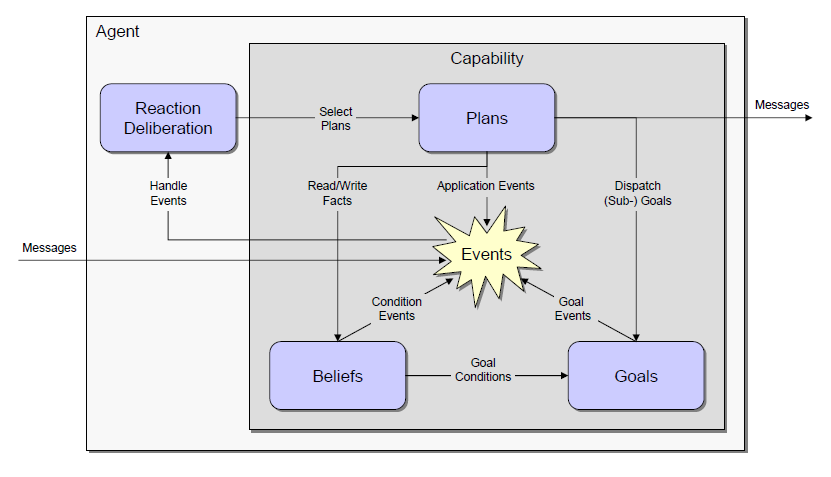
\includegraphics[width=300px]{images/Jadex_agent.png}
	\caption{Jadex abstract agent \cite{pokahr_jadex_2005}}
	\label{fig2}
\end{figure}
\autoref{fig2} depicts an abstract view on a Jadex agent. Every agent may receive messages which trigger internal events that can change his internal knowledge, plans or goals. Interactions with the outside like the environment or other agents happens through the sending of messages. % TODO @manuelmittler I removed the quote as I did not find it to be necessary here. Am I correct that modifications in the environment are also done through messages? -> what do you mean by "modifications in the environment"?
In more detail, beliefs are single facts stored as Java objects which represent the knowledge of an agent. % TODO @manuelmittler should I know, what a fact is? Because I honestly don't.. -> Didn't you attend some logic lectures?
They are stored as key-value pairs.
The advantage of storing information as facts is that the programmer has a central place for the knowledge and can query the agent's beliefs. % TODO @manuelmittler or do you mean that there is an advantage by storing them as Java Objects? -> yes
Monitoring of the beliefs is possible too.

The goals are momentary desires of an agent for which the agent engages into suitable actions until it considers the goal as being reached, unreachable, or not wanted any more.
Jadex distinguishes between four generic goal types.
A perform goal is directly related to the execution of actions.
Therefore, the goal is considered to be reached, when some actions have been executed, regardless of the outcome of these actions.
An achieve goal is a goal in the traditional sense, which defines a desired world state without specifying how to reach it.
Agents may try several different alternative plans, to achieve a goal of this type.
A query goal is similar to an achieve goal, but the desired state is not a state of the (outside) world, but in internal state of the agent, regarding the availability of some information the agent wants to know about.
For goals of type maintain an agents keep track of a desired state, and will continuously execute appropriate plans to re-establish this maintained state whenever needed.
In contrast to goals, events are (per default) dispatched to all interested plans but do not support any BDI-mechanism.
Therefore, the originator of an internal event is usually not interested in the effect the internal event may produce but only wants to inform some interested parties about some occurrence.
Plans represent the behavioural elements of an agent and are composed of a head and a body part.
The plan head specification is similar to other BDI systems and mainly specifies the circumstances under which a plan may be selected, e.g. by stating events or goals handled by the plan and preconditions for the execution of the plan.
Additionally, in the plan head a context condition can be stated that must be true for the plan to continue executing.
The plan body provides a predefined course of action, given in a procedural language.
This course of action is to be executed by the agent, when the plan is selected for execution, and may contain actions provided by the system API, such as sending messages, manipulating beliefs, or creating sub-goals (cf. \cite{braubach_jadex_2004})

Jadex is not based on a new agent programming language.
Instead, a hybrid approach is chosen, distinguishing explicitly between the language used for static agent type specification and the language for defining the dynamic agent behaviour.
An agent in Jadex consists of two components: An \emph{agent definition file} (short: ADF) for the specification of beliefs, goals, and plans as well as their initial values and on the other hand procedural plan code.
\begin{figure}
	\centering
	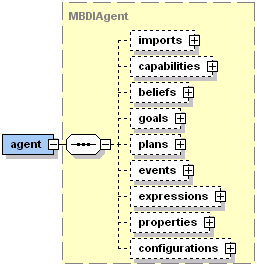
\includegraphics[height=200px]{images/jadexagentadf.png}
  \caption{Jadex top level ADF elements \cite{ActiveComponents}}
	\label{fig3}
\end{figure}
The procedural part of plans (the plan bodies) are realized in an ordinary programming language (Java) and have access to the BDI facilities of an agent through an application interface (API).
The plan body is a standard Java class that extends a predefined Jadex framework class and has at least to implement the abstract body() method which is invoked after plan instantiation.
\begin{lstlisting}
public class ServeCoffeePlanB1 extends Plan {
   // Plan attributes.

   public ServeCoffeePlanB1() {
       // Initialization code.
   }

   public void body() {
       // Plan code.
   }
}
\end{lstlisting}
The plan body is associated to a plan head in the ADF.
This means that in the plan head several properties of the plan can be specified, e.g. the circumstances under which it is activated and its importance in relation to other plans.
\begin{lstlisting}
<agent xmlns="http://jadex.sourceforge.net/jadex-bdi"
 xmlns:xsi="http://www.w3.org/2001/XMLSchema-instance"
 xsi:schemaLocation="http://jadex.sourceforge.net/jadex-bdi
                      http://jadex.sourceforge.net/jadex-bdi-2.0.xsd"
 name="CoffeeAgent">

 <plans>
   <plan name="serve">
     <body class="ServeCoffeePlanB1"/>
     <waitqueue>
       <messageevent ref="request_serving"/>
     </waitqueue>
   </plan>
 </plans>

 <events>
   <messageevent name="request_serving" direction="receive" type="fipa">
     <parameter name="performative" class="String" direction="fixed">
       <value>jadex.bridge.fipa.SFipa.REQUEST</value>
     </parameter>
   </messageevent>
 </events>

 <properties>
   <property name="debugging">false</property>
 </properties>

 <configurations>
   <configuration name="default">
     <plans>
       <initialplan ref="serve"/>
     </plans>
   </configuration>
 </configurations>
</agent>
\end{lstlisting}
There are two types of plans in Jadex.
A \emph{service plan} and a \emph{passive plan}.
The service plan, as the name indicates, is an instance of a plan which waits for service requests.
Therefore a service plan can set up its private event wait queue and receive events for later processing, even when it is working at the moment.
In contrast to that, a passive plan is only running when it has a task to achieve.
For this kind of plan the triggering event and goals must be specified must be specified in the agent definition file to let the agent know what kinds of events this plan can handle.
When an agent receives an event, the BDI reasoning engine builds up the so called applicable plan list which contains all plans that can handle the current event or goal.
The candidates are selected and instantiated for execution.

The execution model for Jadex looks like the following:
\begin{figure}
	\centering
	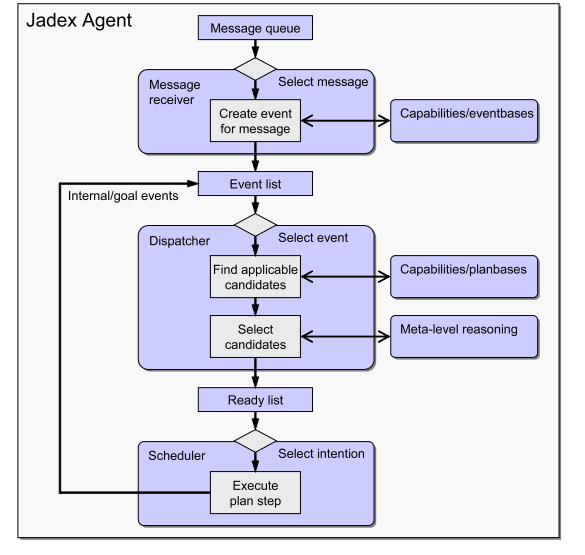
\includegraphics[width=300px]{images/Jadex_execution_model.png}
	\label{fig4}
	\caption{Jadex execution model \cite{pokahr_jadex_2005}}
\end{figure}
\newline
When an agent receives a message it is placed at a message queue.
In the next step the message has to be assigned to a capability, which can handle the message.
A suitable capability is found by matching the message against the event templates defined in the event base of each capability.
The best matching template is then used to create an appropriate event in the scope of the capability.
After that the created event is subsequently added to the agent's global event list.
The dispatcher is responsible for selecting applicable plans for the events from the event list.
After plans have been selected, they are placed in the ready list, waiting for execution.
The execution of plans is performed by a scheduler, which selects plans from the ready list.\cite{pokahr_jadex_2005}

All in all Jadex is a powerful framework that supports easy agent construction with XML-based agent description and procedural plans in Java.
Additionally, it offers tool support for development debugging.
It comes for example with a BDI-Viewer that allows observing and modifying the internal state of an agent and a logger agent that collects log-outputs of any agent.
Judging from this knowledge, Jadex seems suitable for the purpose of competing in the multi-agent programming contest.


\subsubsection[AgentSpeak(L)]{AgentSpeak(L)$^{\circ,\dagger}$}\label{fun:apl_asl}
This section provides an overview of the general concepts of the logic programming language AgentSpeak(L).
The language was developed by Rao~\cite{anand_AgentSpeak_1996}.
Except for the examples, this section takes its information from the cited paper.
The idea behind AgentSpeak(L) was to make the theoretic concept of BDI agents usable in practical scenarios. % 44

The main language constructs are \emph{beliefs}, \emph{goals} and \emph{plans}.
Beliefs represent information that an agent has about its environment.
A belief \texttt{hasCoffee(p)} for example denotes that an agent knows that the person \texttt{p} has coffee.
In AgentSpeak(L), variables are indicated by using a capital first letter whereas terms with a lower-case initial letter are constants. % 45
\begin{lstlisting}[caption={Initial beliefs.}, label=lst:asl_initBeliefs]
  ~hasCoffee(jane).
  ~hasCoffee(john).
\end{lstlisting}
\autoref{lst:asl_initBeliefs} shows the initial beliefs of an agent in the example we just introduced.
The tilde ($\sim$) expresses that the agent knows that neither \texttt{john} nor \texttt{jane} has coffee.
At any given time, the sum of all current beliefs of an agent are called its \emph{belief base}~\cite{bordini_jason_2005}. % p.8

Goals can be divided into \emph{achievement goals} and \emph{test goals}.
The first expresses the wish of an agent to reach a state where a belief holds where the second tests whether a belief holds in the current state.
Beliefs hold when the agent knows they are true or when the variables can be bound to at least one known configuration.
For example, a given achievement goal \texttt{!hasCoffee(p)} means that an agent wants to achieve that person \texttt{p} has coffee.
Similarly, \texttt{?hasCoffee(p)} expresses that an agent tests whether \texttt{p} has coffee.
Hence, this expression will evaluate to true or false depending on the agent's knowledge.
Achievement goals are comparable to desires. % 45
\autoref{lst:asl_initGoal} shows the initial achievement goal which express that the agent wants to have served everyone coffee.
\begin{lstlisting}[firstnumber=3, caption={Initial goal.}, label=lst:asl_initGoal]
  !servedCoffee.
\end{lstlisting}

\emph{Events} are introduced to allow agents to react on changes in their own knowledge or the world.
They can be distinguished into the addition and removal of beliefs or goals.
Additions are denoted by a plus (+) and removals by using a minus (-) sign in front of the goal or belief:
\begin{itemize}
  \item \texttt{+hasCoffee(p)}: an agent is informed that \texttt{p} now has coffee.
  \item \texttt{-hasCoffee(p)}: an agent is informed that \texttt{p} no longer has coffee.
  \item \texttt{+!hasCoffee(p)}: an agent is informed that it wants \texttt{p} to have coffee.
  \item \texttt{-!hasCoffee(p)}: an agent is informed that it no longer wants \texttt{p} to have coffee.
  \item \texttt{+?hasCoffee(p)}: an agent is informed that it should test for the belief.
  \item \texttt{-?hasCoffee(p)}: an agent is informed that it no longer needs to test for the belief.
\end{itemize}
In order to handle new events, an agent will look for a matching plan.

Plans can be seen as programmer-defined agent instructions.
They lead to the execution of actions or the splitting of goals into additional goals.
Plans which an agent wants to execute, are similar to intentions for BDI agents.
They are stored as a set of intentions.
The set of plans generally known to an agent is called the \emph{plan library}~\cite{bordini_jason_2005}.
A plan is triggered by events and is context-sensitive.
This means that the execution of a plan can be restricted to states in where certain beliefs exist.
\autoref{lst:asl_sing} illustrates this by showing when the \texttt{sing} action is being executed.
\autoref{l:asl_trigger} is the triggering event of the plan.
In this case, an agent will consider executing this plan, when it notices that someone is poured coffee.
Hence, this plan is called a \emph{relevant plan}.
The underscore (\texttt{\_}) denotes an anonymous variable similar to its use in Prolog.
Its meaning is that it will match any term.
\autoref{l:asl_context} is the plan's context.
The plan is called an \emph{applicable plan} if the context's beliefs are all known to the agent.
In this particular case, the agent must know that there is no person without coffee indicated by the use of the tilde.
Lastly, \autoref{l:asl_body} contains the body of the plan.
Here, the agent should achieve the goal \texttt{sing}.
This will trigger a new event which calls the plan in \autoref{l:asl_sing}.
As its context is empty, the plan can be executed immediately and evaluates to true as there is no body.
\autoref{l:asl_loop} expresses how the event of someone being poured coffee should be alternatively handled.
As AgentSpeak(L) is interpreted from top to bottom, it will only be seen as an applicable plan, if the former relevant plan did not trigger.
Therefore, if the agent knew that there was still someone left without coffee, it will want to achieve the \texttt{servedCoffee} goal again.
% TODO?: explain that this is a better example and hence we first deal with it instead of servedCoffee
\begin{lstlisting}[firstnumber=4, caption={Events for handling someone being poured a coffee as well as the \texttt{sing} plan.}, label=lst:asl_sing]
  +hasCoffee(_):%\label{l:asl_trigger}%
      ~hasCoffee(_)%\label{l:asl_context}%
      <- !sing.%\label{l:asl_body}%
  +hasCoffee(_)%\label{l:asl_loop}%
      <- !servedCoffee.
  +!sing.%\label{l:asl_sing}%
\end{lstlisting}
% We assume that the implementation of AgentSpeak(L) does not do anything if there is no applicable plan for an event. In \autoref{lst:asl_sing} this would be equal to adding a plan for \texttt{hasCoffee(\_)} without context or body. Given this assumption, the \texttt{pourCoffee}-action is then defined as shown in \autoref{lst:asl_pourCoffee}. \autoref{l:asl_pourCoffee} uses a shortcut operator which extends to \texttt{-hasCoffee(\_); +hasCoffee(X)} \cite{bordini_programming_2007}. % 53
\autoref{lst:asl_serve} contains the plan for serving coffee.
It uses a test goal to pick someone without a coffee as shown in \autoref{l:asl_thirsty}.
The person will be bound to the variable \texttt{X}.
After that, an achievement goal is added to the agent's set of intentions to pour \texttt{X} coffee.
The plan does not feature any context as this minimal example ensures that the goal \texttt{!servedCoffee} will only exist when there actually is a person without coffee.
\begin{lstlisting}[firstnumber=10, caption={Definition of the \texttt{servedCoffee} plan.}, label=lst:asl_serve]
  +!servedCoffee:
      <- ?~hasCoffee(X);%\label{l:asl_thirsty}%
         !pourCoffee(X).%\label{l:asl_pour}%
\end{lstlisting}
\autoref{lst:asl_pour} shows a plan which states that if an agent receives an event to achieve the goal \texttt{!pourCoffee} for some person \texttt{X}, it will pour coffee for \texttt{X}.
Additionally, the knowledge about \texttt{X} not having any coffee is removed in \autoref{l:asl_coffeeless}.
\begin{lstlisting}[firstnumber=14, caption={Definition of the \texttt{pourCoffee} plan.}, label=lst:asl_pour]
  +!pourCoffee(X)
      <- +hasCoffee(X);
         -~hasCoffee(X).%\label{l:asl_coffeeless}%
\end{lstlisting}

As shown, AgentSpeak(L) is another logic programming language for agent programming.
It was specifically designed for developing BDI-agents.
In the next section, an interpreter for this language will be given, which further extends it.


\subsubsection[Jason]{Jason$^\circ$}\label{fun:apl_jason}
This section gives a quick overview of Jason, which is an interpreter for AgentSpeak(L).
All information if not marked differently is taken from Bordini et al.~\cite{bordini_jason_2005}.
Besides being an interpreter, Jason extends AgentSpeak(L) by several concepts.
The most important ones will be discussed in this section.

With Jason, terms can represent more than a constant or a variable.
They can be strings, integer or floating point numbers or lists of terms.
Therefore, more complex programmatic operations and arithmetic expressions are possible with Jason.
Furthermore, Jason introduces annotations.
With these annotations, metadata can be added to triggering events and beliefs.
This metadata can be accessed programmatically.
\autoref{lst:jason_annotations} shows the earlier used initial beliefs with added annotations.
The \texttt{source} annotation is the only one with its meaning predefined by Jason.
It expresses the source of the information.
If an agent determined something itself, the \texttt{source} is \texttt{self}.
Did the agent receive the information as a perception of the environment, then the \texttt{source} will be \texttt{percept}.
The source can also be a constant identifying a different agent if that agent is the source of this information.
With the example given in \autoref{lst:jason_annotations}, an achievement goal \texttt{?\~{}hasCoffee(X)[reliability(Y)]} will bind \texttt{X} to \texttt{john} and \texttt{Y} to \texttt{0.3}.
The \texttt{reliability} has no further meaning unless the value bound to \texttt{Y} is used later.
\begin{lstlisting}[caption={Annotation of beliefs in Jason.}, label=lst:jason_annotations]
  ~hasCoffee(jane)[source(self)].
  ~hasCoffee(john)[source(percept), reliability(0.3)].
\end{lstlisting}

Another concept added to AgentSpeak(L) by Jason is called \emph{internal actions}.
It was first introduced and implemented by Bordini et al.~\cite{bordini_agentspeak_2002}.
Most characteristic for these actions is that they do not affect the environment in which the agents are located in.
This means they have no effect on the external world but only on the internal states of the agents as the name suggests.
Hence, any effects of internal actions occur immediately after the action execution instead of only after the next environment processing cycle.
As a result, internal actions can not only be used within a plan's body but also in its context. % all this information is from p. 1297
Internal actions start with a dot (.) followed by a library identifier, another dot and finally the action name.
Bordini et al.~\cite{bordini_agentspeak_2002} implemented various internal actions which are not identified by any explicitly named library.
These methods reside in the so called \emph{standard library} and omit the library declaration when being called.
An example of this is \texttt{.gte(X,Y)} which returns the truth value of \texttt{X}$\geq$\texttt{Y}.
A realisation of the same function outside the standard library could e.g.\ be called \texttt{.math.gte(X,Y)}.
The standard library is included in Jason.
Furthermore, Jason extends this library by various actions including multiple list operations like sorting or retrieving the minimum.
Developers can write additional internal actions in Java or any other programming language which supports the programming framework Java Native Interface. %11

Arguably, the most important internal action is \texttt{.send}.
This action enables inter-agent communication as initially proposed and implemented by Vierira et al.~\cite{vieira_formal_2007}.
It is structurally based on KQML and FIPA~\cite{fernandez_evaluating_2010}.
A short overview of a FIPA message has been given in \autoref{fun:apl_jadex}.
We pass on presenting the structure of a KQML message here as both are similar and KQML is not further developed~\cite{obrien_fipatowards_1998}.
\begin{lstlisting}[caption={Parameters of the internal action \texttt{.send} and an example.}, label=lst:jason_send]
  .send(Receiver, Illocutionary_force, Message_content).%\label{l:jason_send}%
  .send([agent1, agent2], tell, ~hasCoffee(john)).%\label{l:jason_sendInstance}%
\end{lstlisting}
In \autoref{l:jason_send} of \autoref{lst:jason_send} the structure of the \texttt{.send} action is shown.
\autoref{l:jason_sendInstance} shows example usage of this action.
The \texttt{Receiver} is the identifying name or a list of identifying names for the agent(s) to which the message should be addressed to.
The \texttt{Illocutionary\_force} is a constant that specifies what all recipients should do with the message.
It can be:
\begin{itemize}
  \item \texttt{tell}: add the \texttt{Message\_content} to the recipient's belief base.
  \item \texttt{untell}: remove the \texttt{Message\_content} from the recipient's belief base.
  \item \texttt{achieve}: add the \texttt{Message\_content} as an achievement goal to the recipient.
  \item \texttt{unachieve}: make the recipient remove the achievement goal \texttt{Message\_content}.
  \item \texttt{tellHow}: \texttt{Message\_content} is added to the recipient's plan library.
  \item \texttt{untellHow}: \texttt{Message\_content} is removed from the recipient's plan library.
  \item \texttt{askIf}: asks if \texttt{Message\_content} is in the recipient's belief base.
  \item \texttt{askOne}: asks for the first belief matching \texttt{Message\_content}.
  \item \texttt{askAll}: asks for all beliefs matching \texttt{Message\_content}.
  \item \texttt{askHow}: demand all plans a recipient has that match the triggering event given in the \texttt{Message\_content}.
\end{itemize}
Jason automatically processes the messages as needed when a message arrives at an agent\todo{should we explicitly talk about an agent's inbox? Compare with @adaudrich's mentioning of the inbox!}.
A developer can override Jason's default behaviour if further or different processing is desired.
Jason also automatically adds \texttt{source} annotations.
This allows agents to determine the sender of any received message.

There is special support for defining environments with Jason.
Instead of having to do this in AgentSpeak(L), it can be done in Java.
For doing so, a developer has to extend the \texttt{Environment} class and specify the \texttt{getPercepts(String agentName)} and \texttt{executeAction(String agentName, Term action)} methods.
The first method must return a list of literals restricted to what the agent identified by \texttt{agentName} can perceive.
When the second method is called, the programmer must specify how the given \texttt{action} affects the environment.
It returns a boolean to indicate whether the execution was successful.
Such an action can fail if for example a Repairer agent would try to execute the \texttt{attack} action, which it cannot according to the rules specified for the \mars scenario.
To call the \texttt{executeAction} method from an agent, all it has to do is execute e.g. \texttt{attack}.
Jason will then call \texttt{executeAction(String agentName, Term action)} with the parameters bound to the agent's name and the \texttt{attack} action.
For the MAPC itself, no fully simulated environment is needed.
Instead, it is enough to delegate the actions to the MAPC server and process the server replies by returning the transmitted percepts to the respective agents.
Therefore, percepts do not have to be modelled or modified in the environment developed with Jason itself.

Jason also allows running multi-agent systems over networks in a distributed manner.
Hence, the workload can be distributed over multiple machines.
SACI~\cite{hubner_saci_2000} and JADE are the two fully implemented distributed architectures usable out of the box with Jason \cite{bordini_programming_2007}.
Fernández et al.~\cite{fernandez_evaluating_2010} could not prove the intended performance benefits.
The authors tested both SACI and JADE with Jason where one host would run the environment and the other one the agents.
They increased both the amount of agents as well as the size of the environment.
Fernández et al.~\cite{fernandez_evaluating_2010} saw that with increasing complexity, the system became slower compared to when agents and the environment were run on a single machine.
This was due to the added communication cost between the two hosts although connected by Gigabit Ethernet.
As a result, a distributed infrastructure with Jason is only advisable, if the workload cannot be handled by one host alone.
In our case, replying in time has such an importance that trying to keeping the workload processable by one host alone would be the preferred strategy.


\subsubsection[Choice of a programming language.]{Choice of a programming language.$^{\circ/\odot}$}\label{fun:apl_choice}
Based on the previous sections, this section summarises why we chose Jason for developing our agents.
Generally, we could have started from scratch without using a designated agent programming language.
We decided against this idea because of our inexperience with agent programming and artificial intelligence in general.
The fear was to overlook difficulties in the beginning which would later force us to spend more time on fixing mistakes we made in the beginning than on the actual agent development.
To prevent this, we were interested in using an already developed and approved agent programming language.

Given the Mars scenario, Jason can be used to implement a suitable multi-agent system.
In fact, two teams successfully participated in the 2013 Multi-Agent Programming Contest by using Jason \cite{ahlbrecht_multi_2013}. % p.367
Yet, there was no competing team using Jadex or FLUX.
This is of interest because the scenario of 2013 is comparable to the scenario of 2014 \cite{ahlbrecht_mapc_2014}. % p.1,9
As the whole team was inexperienced with logical programming prior to this research lab, being able to develop the environment and some operations via internal actions in Java was beneficial.
Furthermore, the contest organisers provided a Java library which would simplify the communication with their server.
Instead of having to manually compile XML messages and parse the XML server replies, this library allowed simple method calls for server interaction.
Thus, deciding against FLUX meant not having to implement the communication with the server ourselves.
The library would also have been usable with Jadex.
But just like Flux, Jadex does not assist the developer in modelling the environment like Jason does.
Jason's support for environments allowed us to focus more on agent programming
There, we preferred Jason and Jadex over FLUX, because these two languages are built around BDI, which we found to be a clearer structuring of agents.
FLUX on the other hand serves as a quite generic approach to programming multi-agent systems.
Besides the support for developing environments, Jason and Jadex are also different in the way how the initial beliefs, goals and plans are being programmed.

\todo{integrate the text below:}
The difference lies in the storing of beliefs, goals and plans.
In Jadex they are stored in the agent definition file (XML) while in Jason they are stored as facts within the Jason belief base.
Another slight difference is that in Jadex plans have to be written in Java whereas in Jason the programmer can use a combination of Java and AgentSpeak with internal actions.
We did not choose Jadex for our research lab because of the overhead that comes with the XML-syntax.

